% Itt kezdődik a dolgozat lényegi része, úgy értve, hogy a saját munka bemutatása.
% Jellemzően ebben szerepelni szoktak blokkdiagramok, a program struktúrájával foglalkozó leírások.
% Ehhez célszerű UML ábrákat (például osztály- és szekvenciadiagramokat) használni.

% Amennyiben a dolgozat inkább kutatás jellegű, úgy itt lehet konkretizálni a kutatási módszertant, a kutatás tervezett lépéseit, az indoklást, hogy mit, miért és miért pont úgy érdemes csinálni, ahogyan az a későbbiekben majd részletezésre kerül.

% Ebben a fejezetben az implementáció nem kell, hogy túl nagy szerepet kapjon.
% Ez még csak a tervezési fázis.
% (Nyilván ha olyan a téma, hogy magának az implementációnak a módjával foglalkozik, adott formális nyelvet mutat be, úgy a kódpéldákat már innen sem lehet kihagyni.)

% \Section{Táblázatok}

% Táblázatokhoz a \texttt{table} környezetet ajánlott használni.
% Erre egy minta \aref{tab:minta}. táblázat.
% A hivatkozáshoz az egyedi \texttt{label} értéke konvenció szerint \texttt{tab:} prefixszel kezdődik.

% \begin{table}[h]
% \centering
% \caption{Minta táblázat. A táblázat felirata a táblázat felett kell legyen!}
% \label{tab:minta}
% \begin{tabular}{l|c|c|}
% a & b & c \\
% \hline
% 1 & 2 & 3 \\
% 4 & 5 & 6 \\
% \hline
% \end{tabular}
% \end{table}

% \Section{Ábrák}

% Ábrákat a \texttt{figure} környezettel lehet használni.
% A használatára egy példa \aref{fig:cimer}. ábrán látható.
% Az \texttt{includegraphics} parancsba 
% Az ábrák felirata az ábra alatt kell legyen.
% Az ábrák hivatkozásához használt nevet konvenció szerint \texttt{fig:}-el célszerű kezdeni.

% \begin{figure}[h]
% \centering
% 
\includegraphics[scale=0.3]{images/me_logo.png}
% \caption{A Miskolci Egyetem címere.}
% \label{fig:cimer}
% \end{figure}

% \Section{További környezetek}

% A matematikai témájú dolgozatokban szükség lehet tételek és bizonyításaik megadására.
% Ehhez szintén vannak készen elérhető környezetek.

% \begin{definition}
% Ez egy definíció
% \end{definition}

% \begin{lemma}
% Ez egy lemma
% \end{lemma}

% \begin{theorem}
% Ez egy tétel
% \end{theorem}

% \begin{proof}
% Ez egy bizonyítás
% \end{proof}

% \begin{corollary}
% Ez egy tétel
% \end{corollary}

% \begin{remark}
% Ez egy megjegyzés
% \end{remark}

% \begin{example}
% Ez egy példa
% \end{example}

\colorlet{punct}{red!60!black}
\definecolor{background}{HTML}{EEEEEE}
\definecolor{delim}{RGB}{20,105,176}
\colorlet{numb}{magenta!60!black}

\Chapter{Tervezés}

% TODO: Érdemes lenne részletezni magát az adatmodellt is, tehát hogy egy felhasználóhoz, feladathoz mik tartoznak. (Lehet a felületi tervek előtt vagy után is, szokták így-is úgy-is.)

\Section{Kinézet}
A kinézetet játékos, egyszerű és átláthatóra szeretném csinálni.
Mindenhol játékos ikonokat és színvilágot szeretnék használni, az oldal ikonja az alábbi lenne:

\begin{figure}[h]
    \centering
    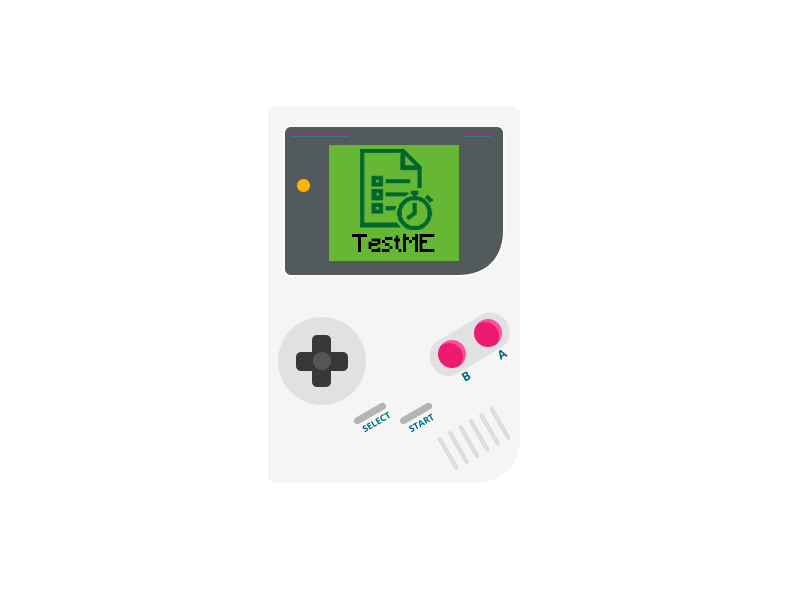
\includegraphics[height=5cm]{images/gameboy.png}
\end{figure}


Minden grafikus elem szeretném hogy egységes legyen így törekedtem arra hogy hasonló stílusú legyen minden. Az egyéb funkciókhoz vagy oldalakhoz társított ikonok, amelyek az oldalt még játékosabbá tennék pedig az alábbiak lennének:

\begin{figure}[h]
    \begin{subfigure}{.1\textwidth}
        \centering
        
\includegraphics[width=.8\linewidth]{images/icons/003-swords.png}
    \end{subfigure}
    \begin{subfigure}{.1\textwidth}
        \centering
        
\includegraphics[width=.8\linewidth]{images/icons/005-fists.png}
    \end{subfigure}
    \begin{subfigure}{.1\textwidth}
        \centering
        
\includegraphics[width=.8\linewidth]{images/icons/006-gamer.png}
    \end{subfigure}
    \begin{subfigure}{.1\textwidth}
        \centering
        
\includegraphics[width=.8\linewidth]{images/icons/007-gamer.png}
    \end{subfigure}
    \begin{subfigure}{.1\textwidth}
        \centering
        
\includegraphics[width=.8\linewidth]{images/icons/014-computer.png}
    \end{subfigure}
    \begin{subfigure}{.1\textwidth}
        \centering
        
\includegraphics[width=.8\linewidth]{images/icons/028-trophy.png}
    \end{subfigure}
    \begin{subfigure}{.1\textwidth}
        \centering
        
\includegraphics[width=.8\linewidth]{images/icons/030-flag.png}
    \end{subfigure}
    \begin{subfigure}{.1\textwidth}
        \centering
        
\includegraphics[width=.8\linewidth]{images/icons/052-rank.png}
    \end{subfigure}
    \begin{subfigure}{.1\textwidth}
        \centering
        
\includegraphics[width=.8\linewidth]{images/icons/053-sword.png}
    \end{subfigure}
    \begin{subfigure}{.1\textwidth}
        \centering
        
\includegraphics[width=.8\linewidth]{images/icons/054-sword.png}
    \end{subfigure}
    \begin{subfigure}{.1\textwidth}
        \centering
        
\includegraphics[width=.8\linewidth]{images/icons/057-computer.png}
    \end{subfigure}
    \begin{subfigure}{.1\textwidth}
        \centering
        
\includegraphics[width=.8\linewidth]{images/icons/058-potion.png}
    \end{subfigure}
\end{figure}

Az ikonokat a Flaticon nevű oldalról töltöttem le \ref{competitiveGamingIcon}.
% TODO: Leírni, hogy az ikonok honnan származnak.

Valamint Bootstrap-et szeretnék használni ami egy olyan keretrendszer, amely segít a weboldalak gyorsabb és könnyebb megtervezésében. HTML és CSS alapú tervezősablonokat tartalmaz a tipográfiához, űrlapokat, gombokat, táblázatokat, navigációt, modelleket stb. Ez segítene abban hogy az oldalon egységes kinézetet hozhassak létre valamit a Bootstrap CSS-je alkalmazkodik a telefonokhoz, táblagépekhez és asztali számítógépekhez is.

Ehhez egy ingyenes Bootstrap témát választottam ami szerintem menne a weboldal témájához, ezt a témát Litera-nak\ref{litera} hívják.

\Section{Az oldal felépítése}

A funkciók elrendezésének és felépítésének bemutatására képernyőterv vázlatot (magyarul drótváznak, angolul wireframe vagy mockup-nak is nevezzük) készítettem a MockFlow \ref{mockflow} nevű oldalon.
Először azt az oldalt mutatom be amivel mindenki először találkozik az oldal megnyitásakor, ez pedig a bejelentkezési és regisztrációs felület.

\subsection{Bejelentkezés és regisztráció}

\begin{figure}[H]
    \centering
    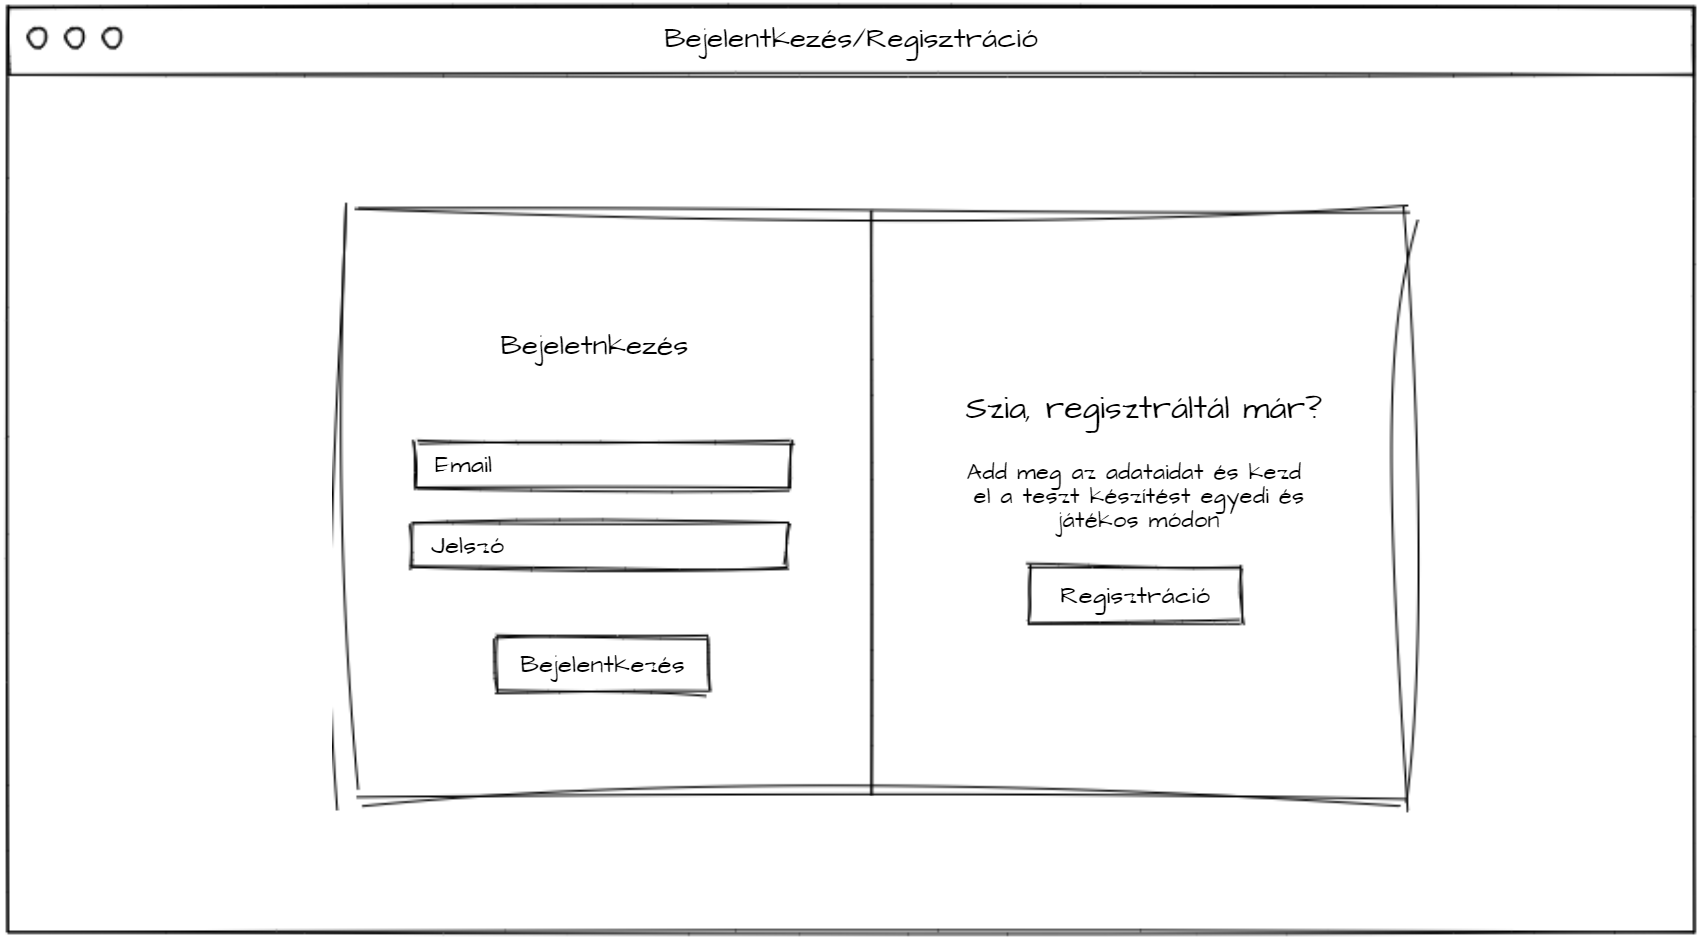
\includegraphics[width=\linewidth]{images/login_wireframe.png}
    \caption{Bejelentkezés}
    \label{fig:login_wireframe}
\end{figure}

\begin{figure}[H]
    \centering
    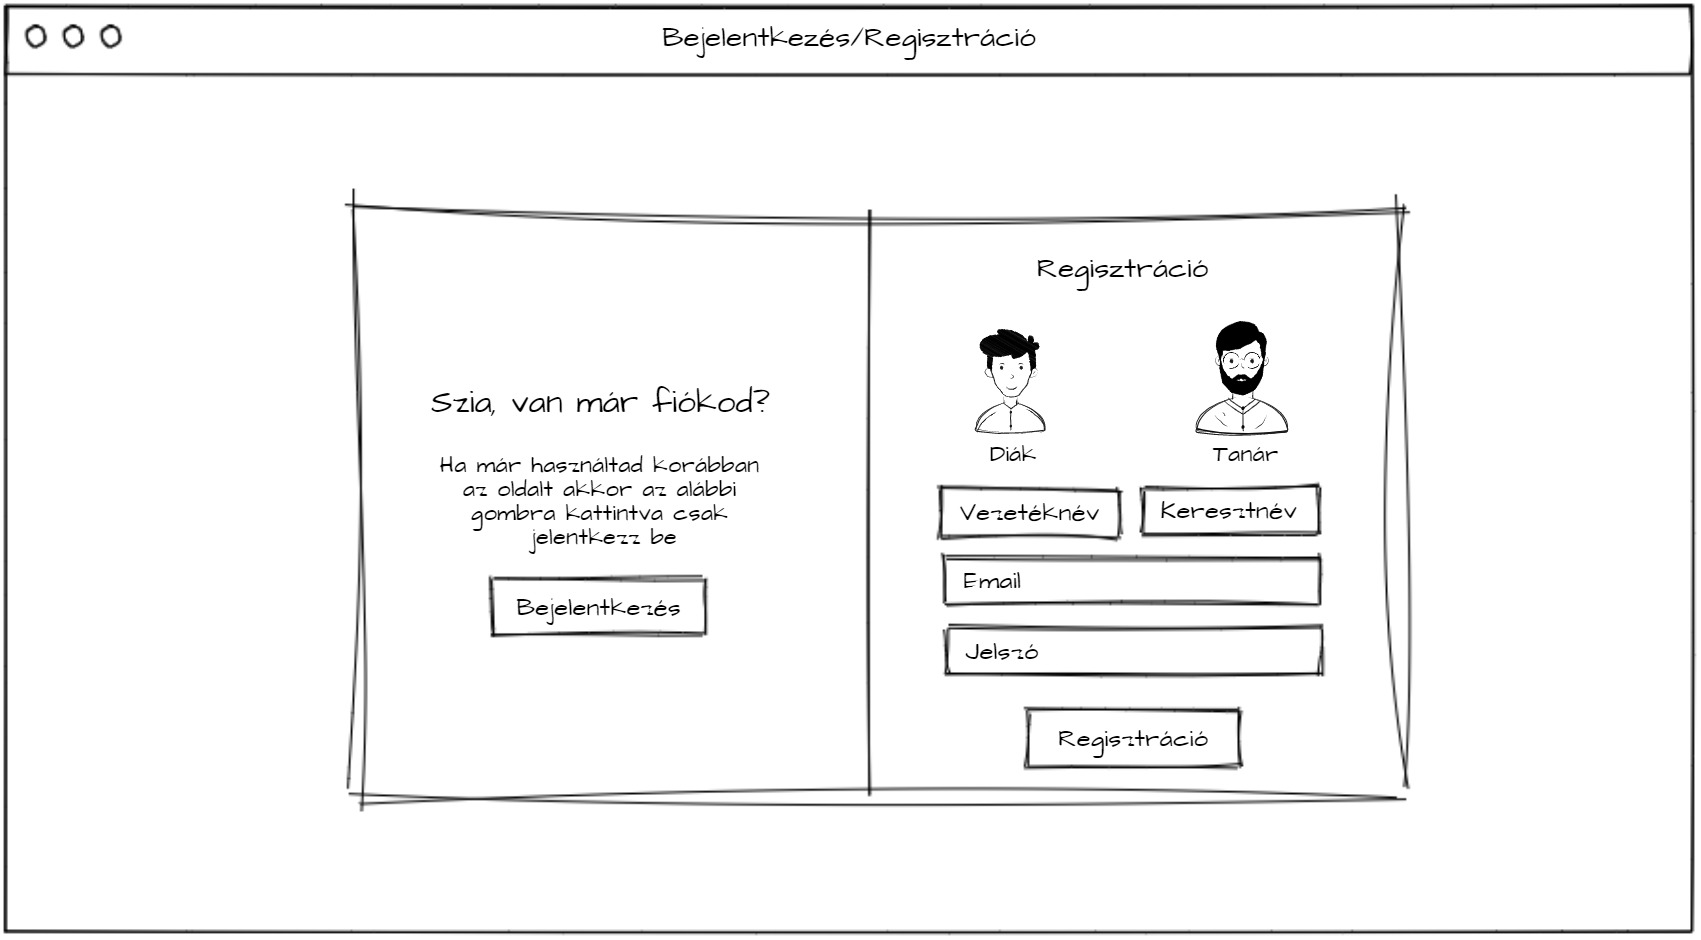
\includegraphics[width=\linewidth]{images/signin_wireframe.png}
    \caption{Regisztráció}
    \label{fig:signin_wireframe}
\end{figure}

Bejelentkezni \ref{fig:login_wireframe} email cím és jelszóval lehet. Regisztrációkor \ref{fig:signin_wireframe} pedig ki kell választani hogy tanár vagy diákként szeretnénk regisztrálni majd meg kell adni az alapvető adatokat.
Ezután ha sikeresen beléptünk vagy regisztráltunk akkor hozzáférhetünk az oldalhoz.

\subsection{Főoldal}

\begin{figure}[H]
    \centering
    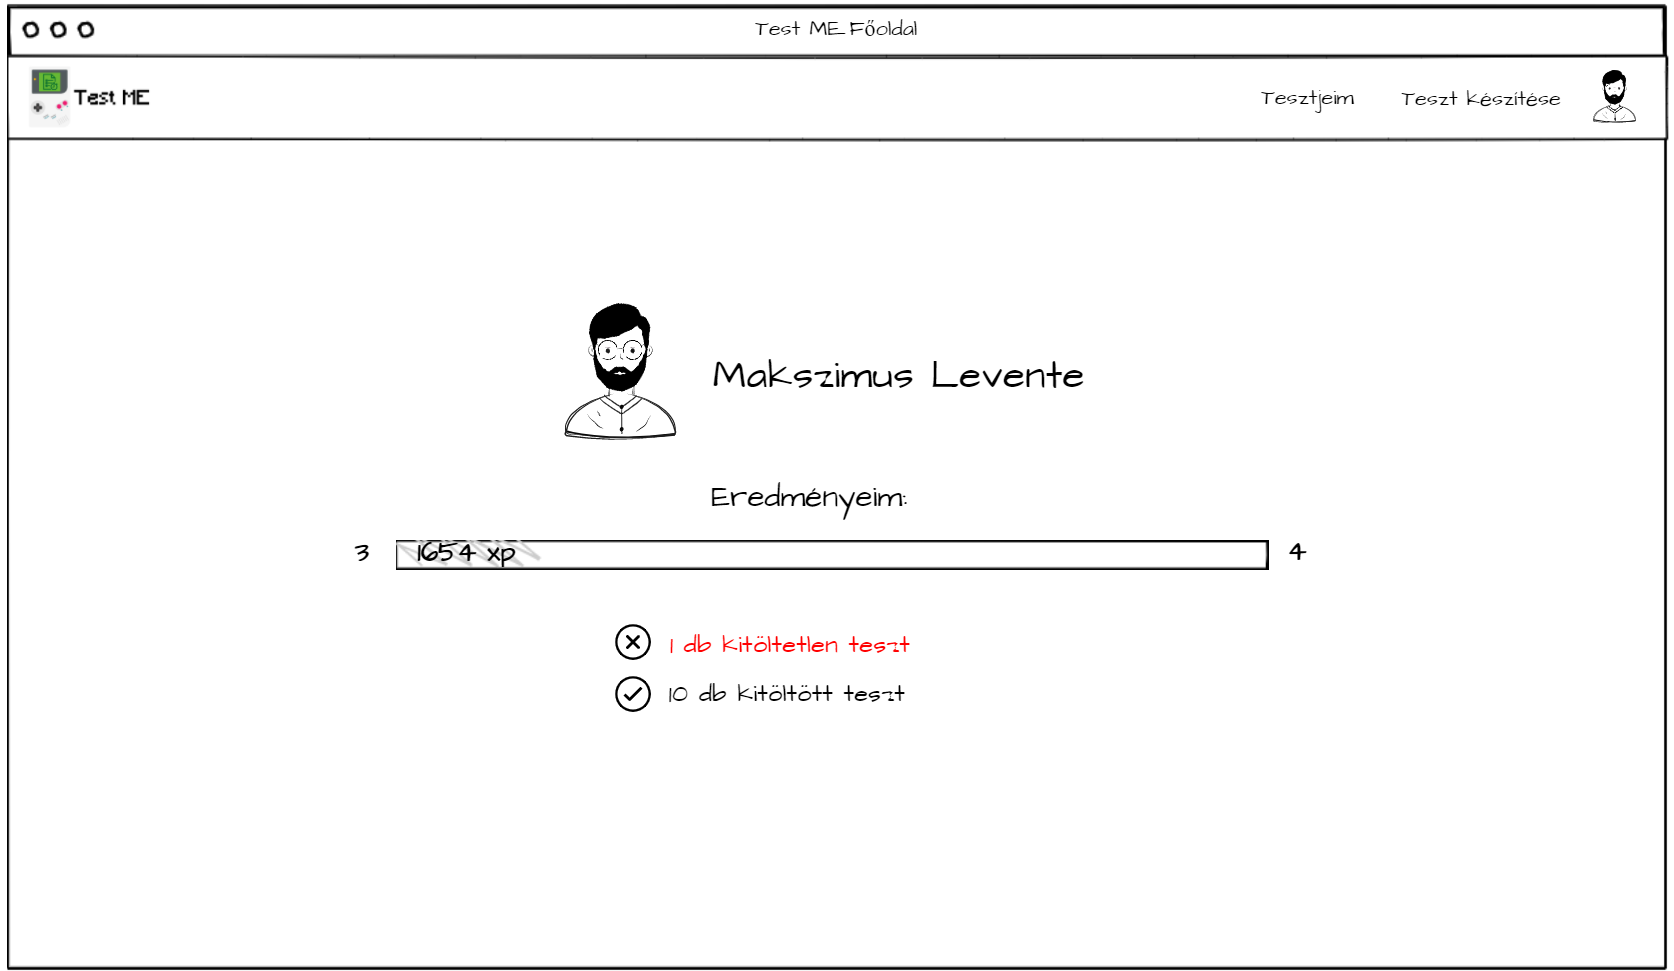
\includegraphics[width=\linewidth]{images/main_login_wireframe.png}
    \caption{Főoldal}
    \label{fig:main_page}
\end{figure}

Itt láthatjuk \ref{fig:main_page} a felhasználónevünket, hogy mennyi xp-vel rendelkezünk, hanyas szintűek vagyunk, és hogy hány darab kitöltött és kitöltetlen tesztünk van még.

\subsection{Teszt készítés}

\begin{figure}[H]
    \centering
    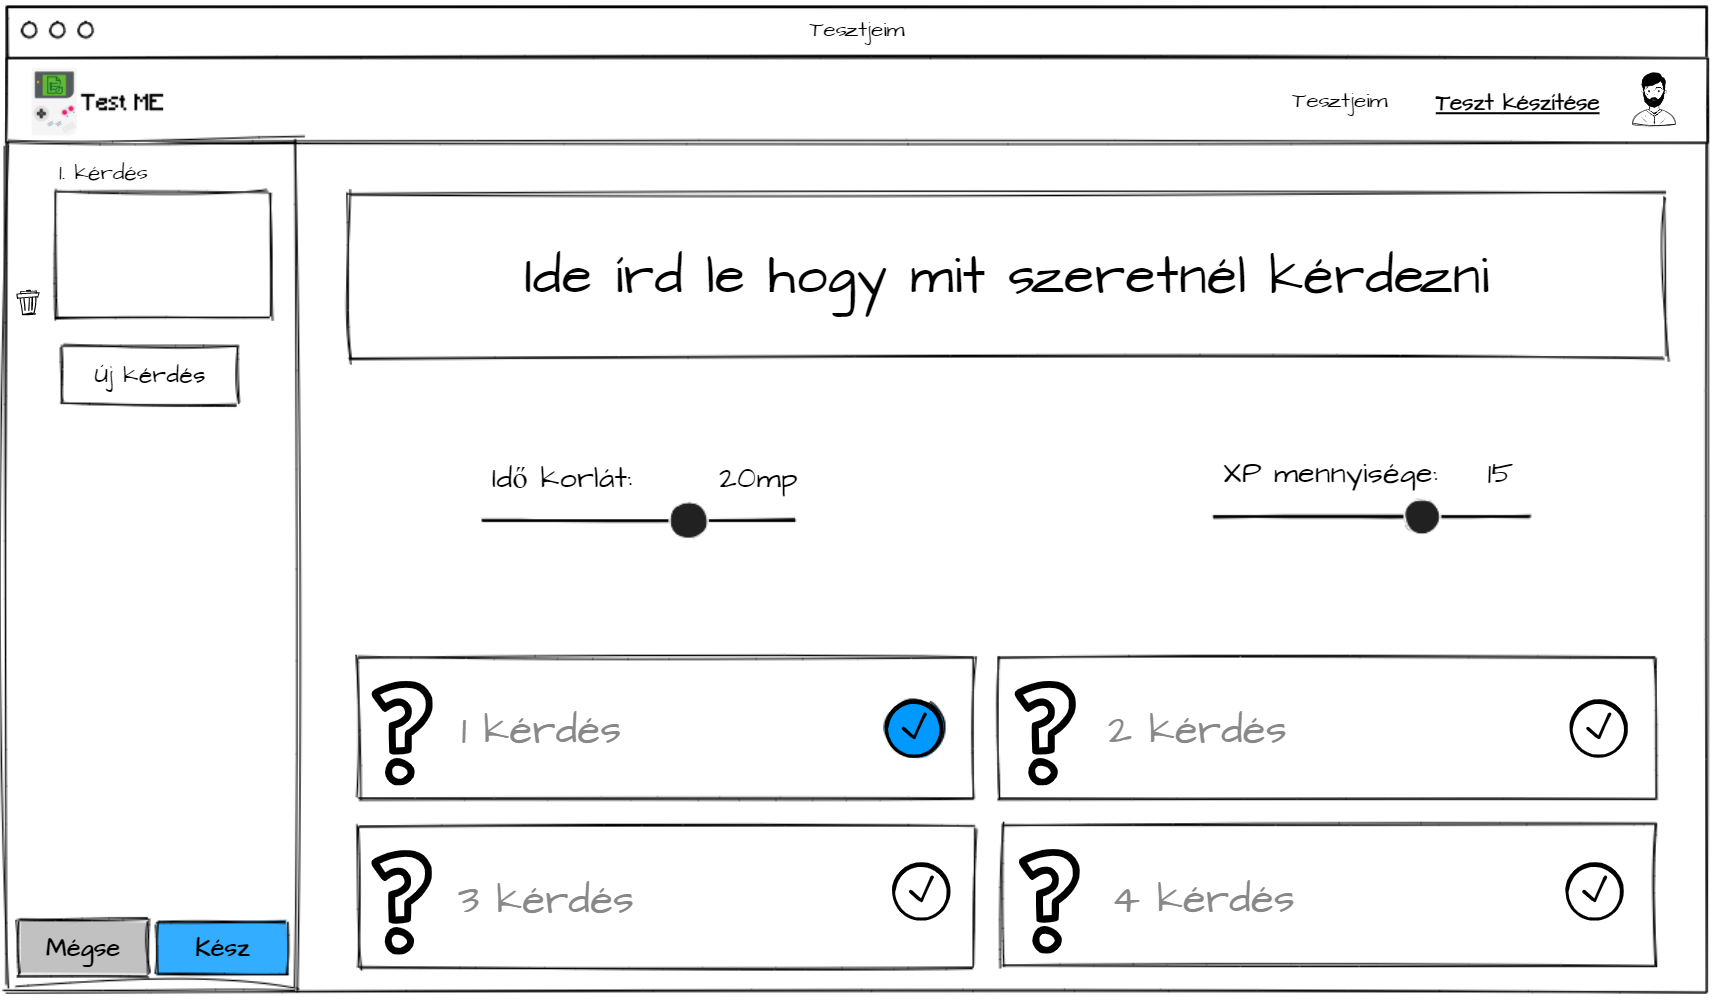
\includegraphics[width=\linewidth]{images/make_test_wireframe.png}
    \caption{Kvíz teszt készítés}
    \label{fig:new_quiz_question}
\end{figure}

Ezen a képen \ref{fig:new_quiz_question} a tesztkészítési felület látható amelyhez majd csak a tanárok férhetnek hozzá. Egy tesztnél meghatározható hogy mi legyen a kérdés, mennyi idő legyen rá, mennyi jutalmat lehessen érte kapni, vagyis xp-t és hogy mik legyenek a válaszok és azok közül melyik a jó.


\begin{figure}[H]
    \centering
    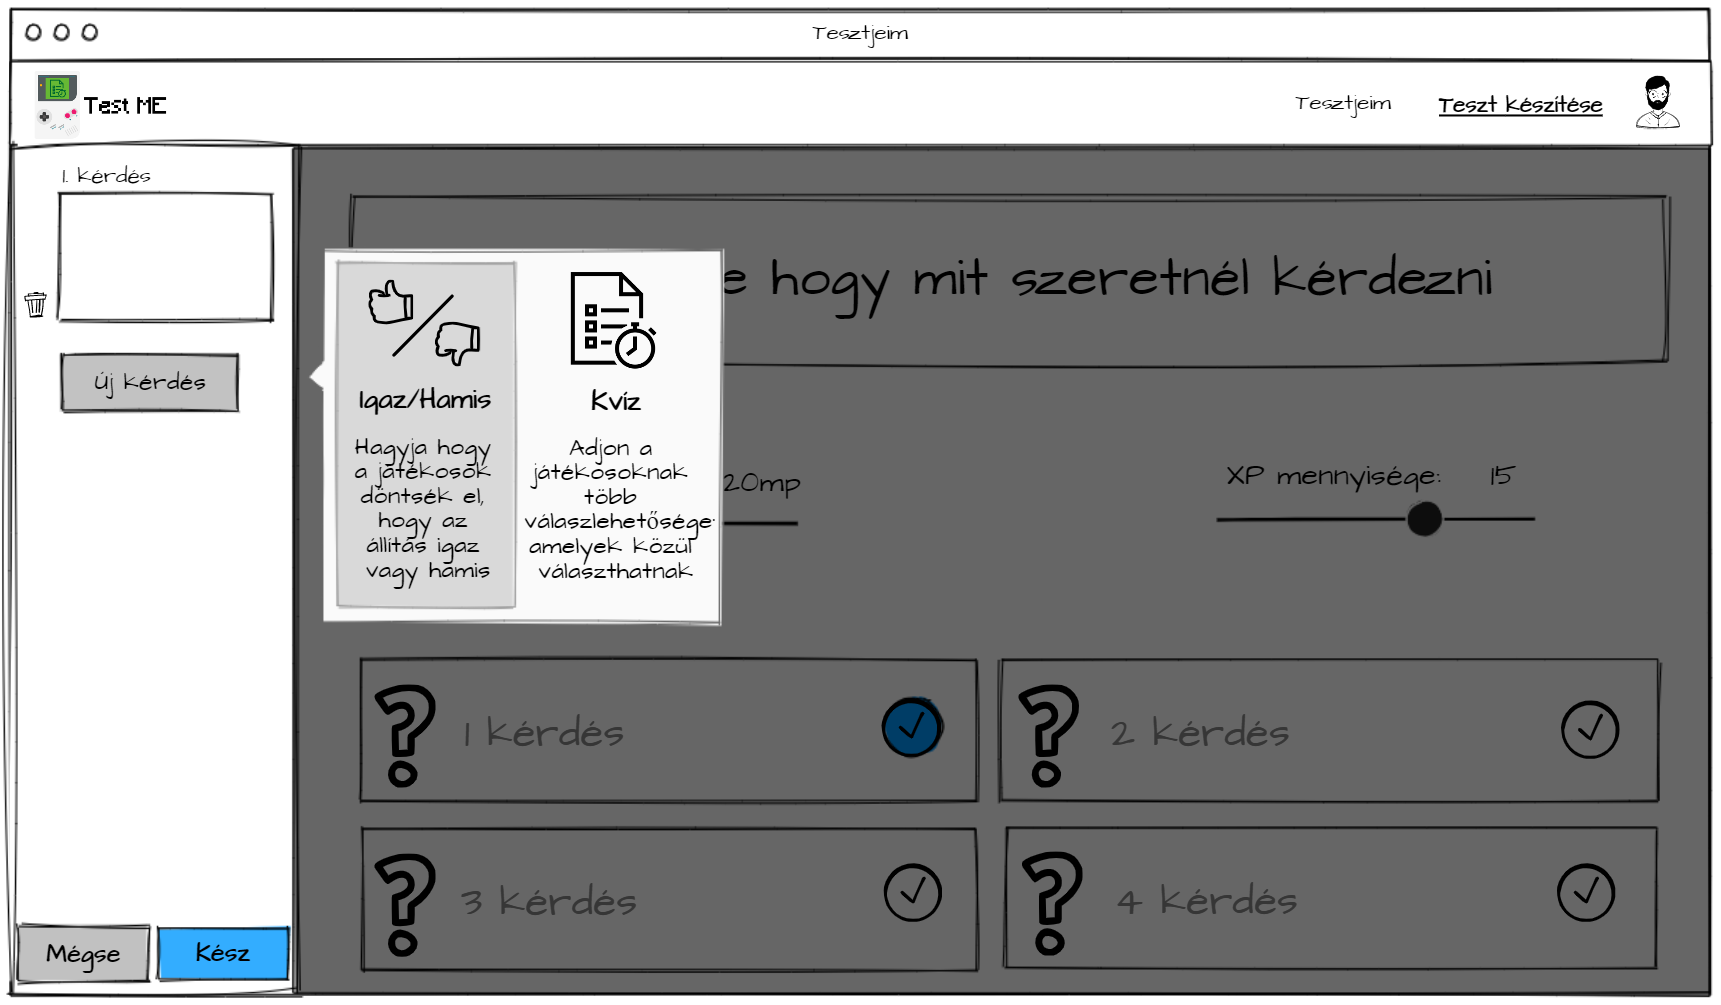
\includegraphics[width=\linewidth]{images/make_test2_wireframe.png}
    \caption{Új kérdés hozzáadása}
    \label{fig:new_question}
\end{figure}

Ezután ha elkészítettünk egy kérdést az "Új kérdés" gomb megnyomásával lehet majd új kérdést hozzáadni, itt választhatunk hogy igaz/hamis vagy kvíz típusú kérdést szeretnénk feltenni \ref{fig:new_question}.

\begin{figure}[H]
    \centering
    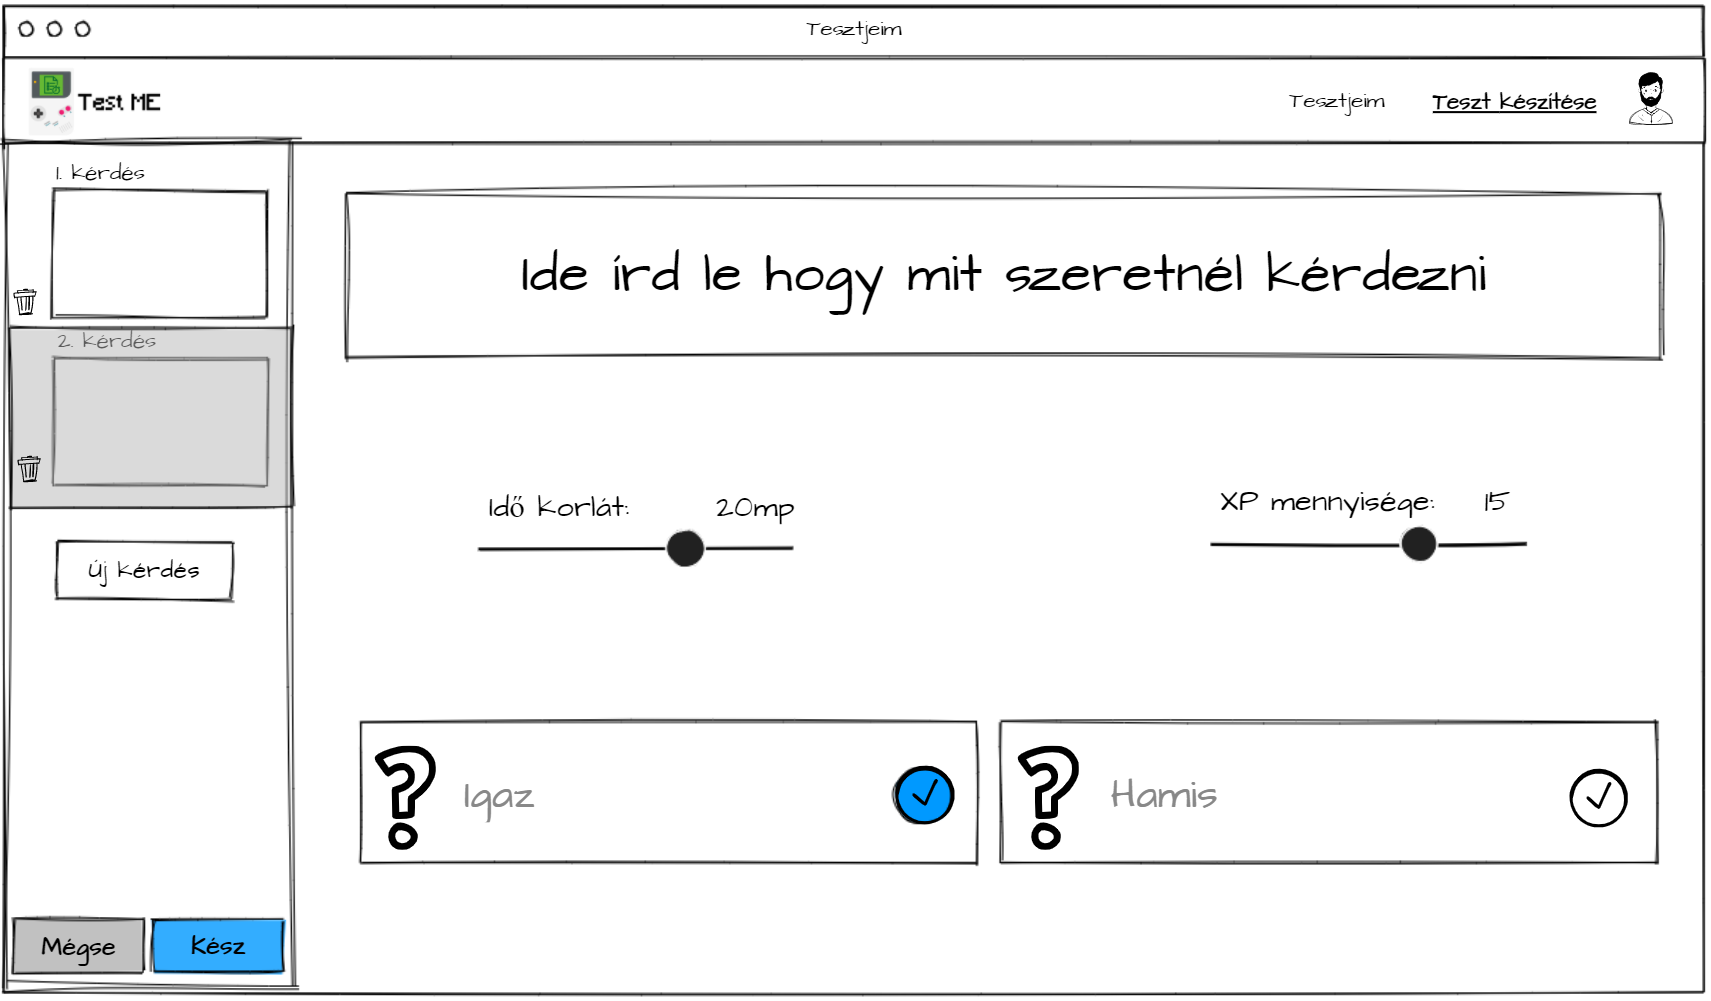
\includegraphics[width=\linewidth]{images/make_test3_wireframe.png}
    \caption{Igaz/hamis teszt készítése}
    \label{fig:test_true_false}
\end{figure}

Az igaz/hamis típusú kérdésnél csak annyi változik hogy nem lehet válasz lehetőséget írni csak azt hogy az állítás igaz vagy hamis \ref{fig:test_true_false}.

\begin{figure}[H]
    \centering
    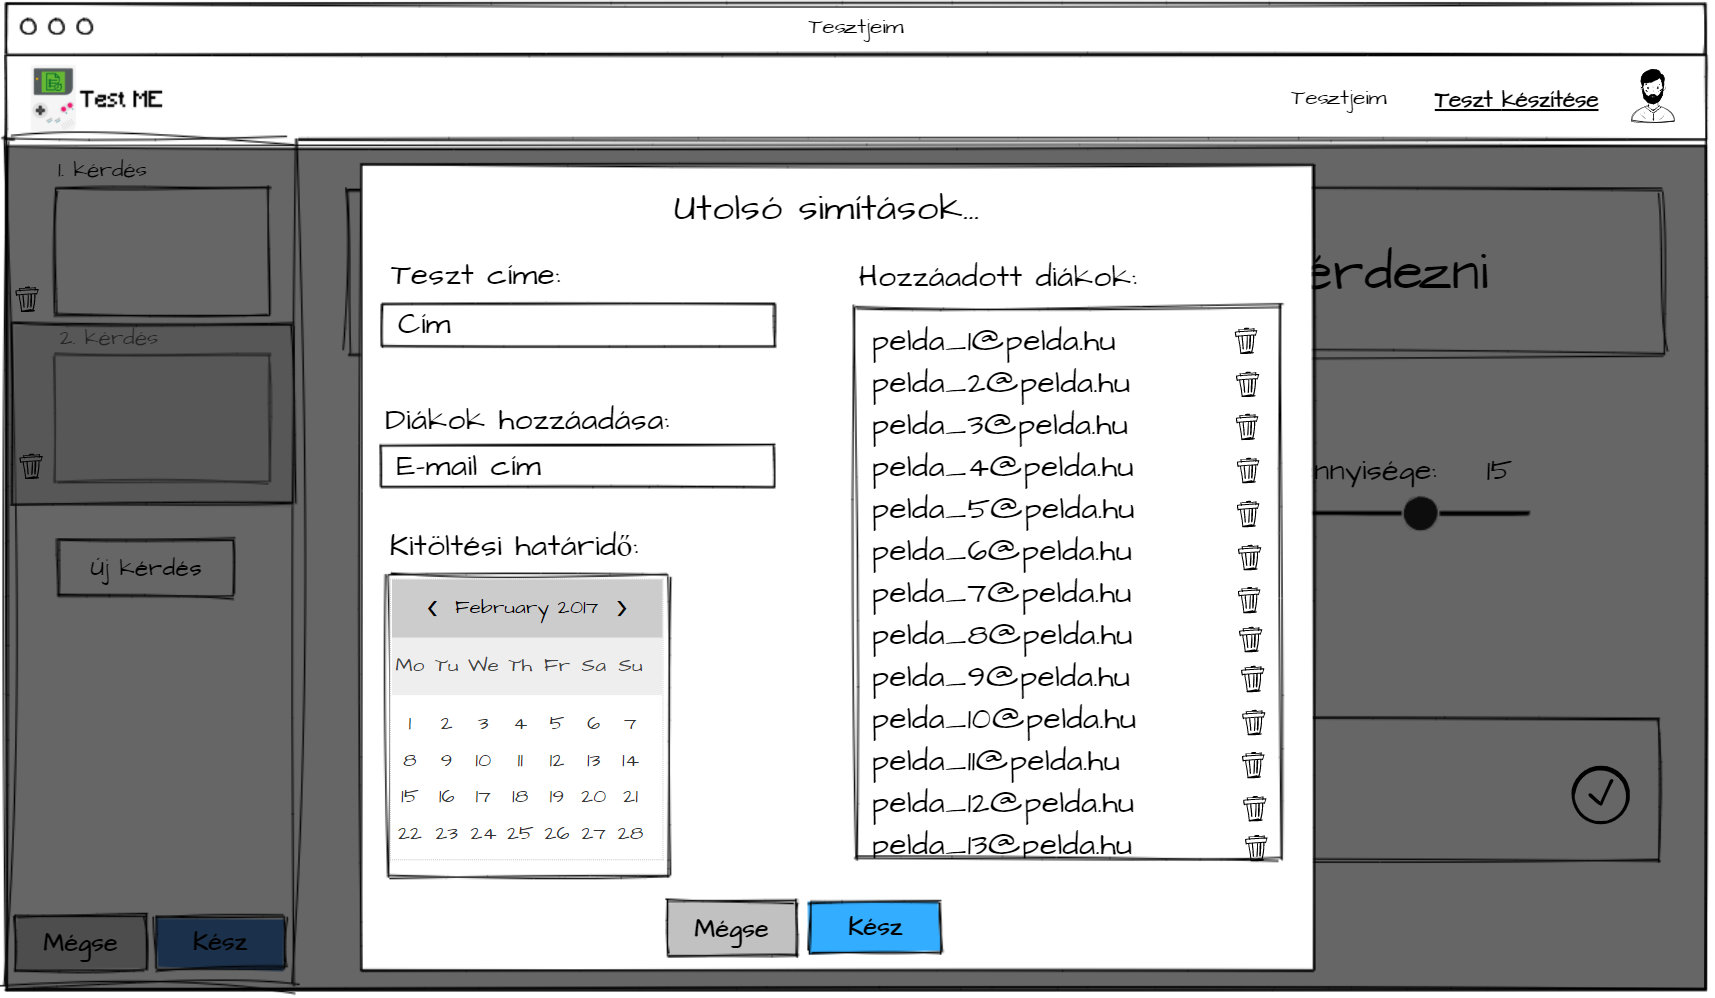
\includegraphics[width=\linewidth]{images/make_test4_wireframe.png}
    \caption{Adatok megadása és teszt elmentése}
    \label{fig:save_test}
\end{figure}

Az utolsó lépés pedig az hogy adunk címet a tesztnek, ilyen névvel fog megjelenni majd a diákoknak. Ezután hozzáadunk tetszőleges számú diákot akiktől szeretnénk hogy töltsék ki majd, egy kitöltési határidőt, és elkészült a tesztünk \ref{fig:save_test}.

\subsection{Saját tesztek}
\begin{figure}[H]
    \centering
    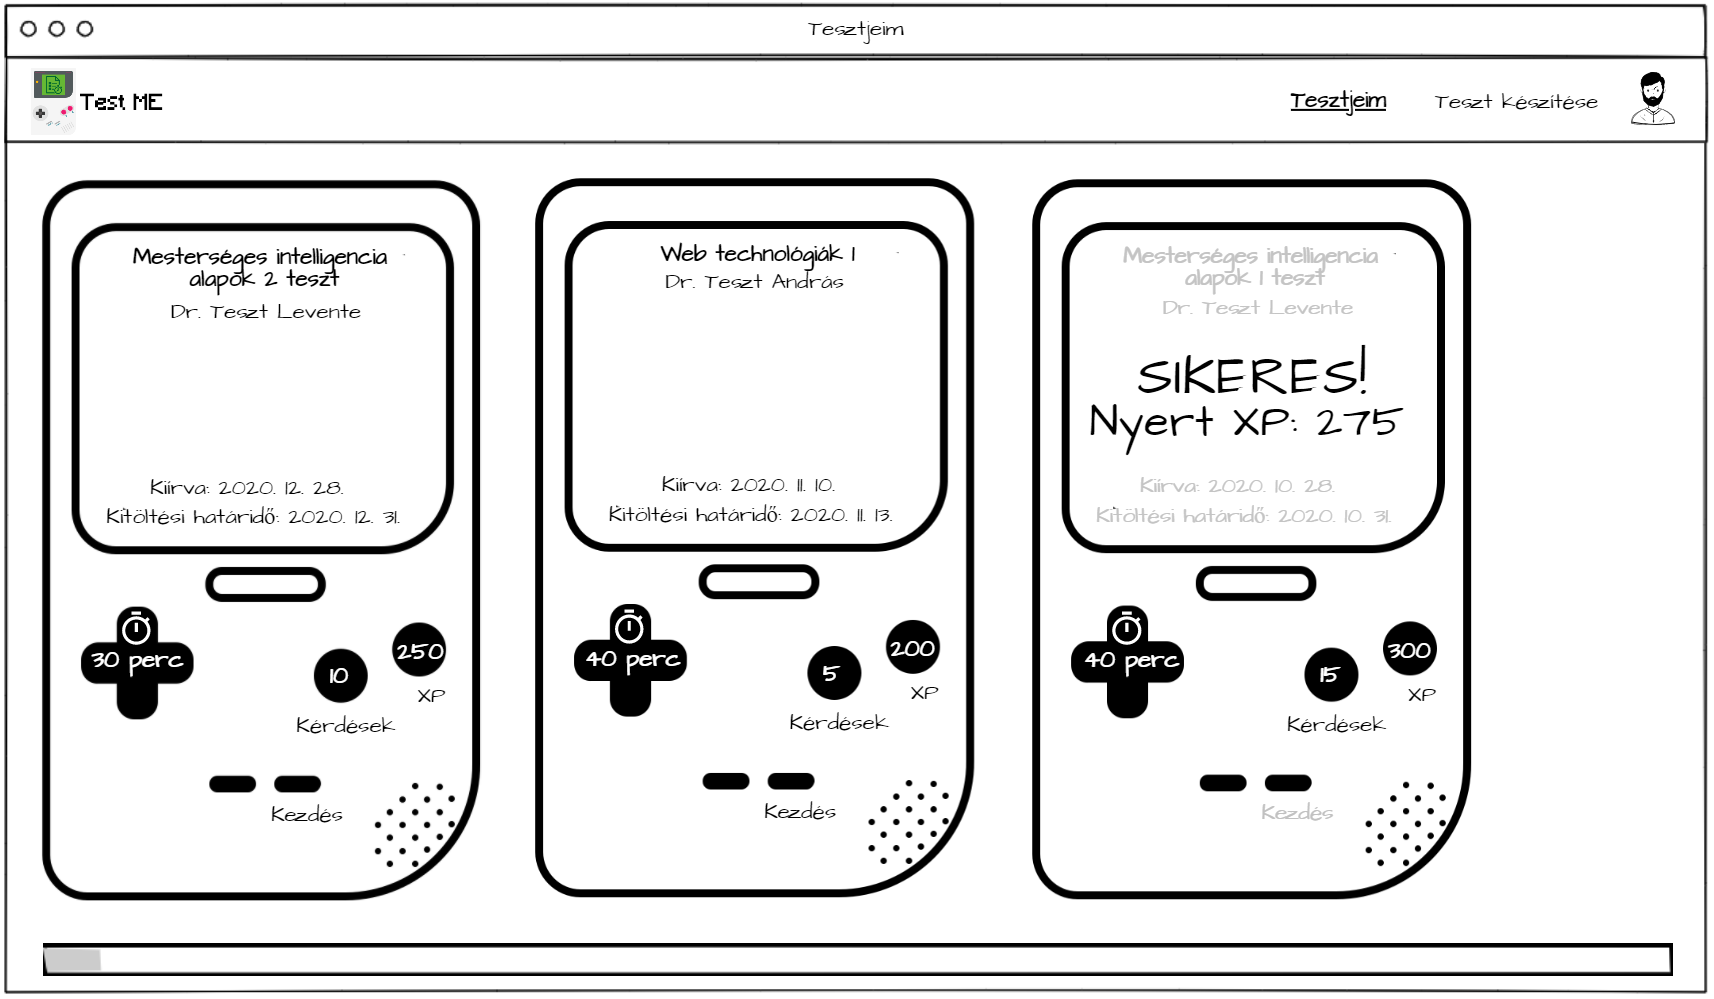
\includegraphics[width=\linewidth]{images/my_tests_wireframe.png}
    \caption{Felhasználóhoz rendelt tesztek}
    \label{fig:my_tests}
\end{figure}

Ezen a képen \ref{fig:my_tests} a diákhoz rendelt teszteket látjuk. Itt azok az adatok láthatóak amiket tesztkészítéskor adott meg a tanár. Tehát a kitöltési határidő, mi a teszt címe, mennyi idő van rá, hány kérdés van és hogy mennyi pontot lehet szerezni. Ezenkívül láthatjuk még hogy mikor lett kiírva és egy kezdés gombot amivel kitölthetjük.

\subsection{Teszt kitöltése}

\begin{figure}[H]
    \centering
    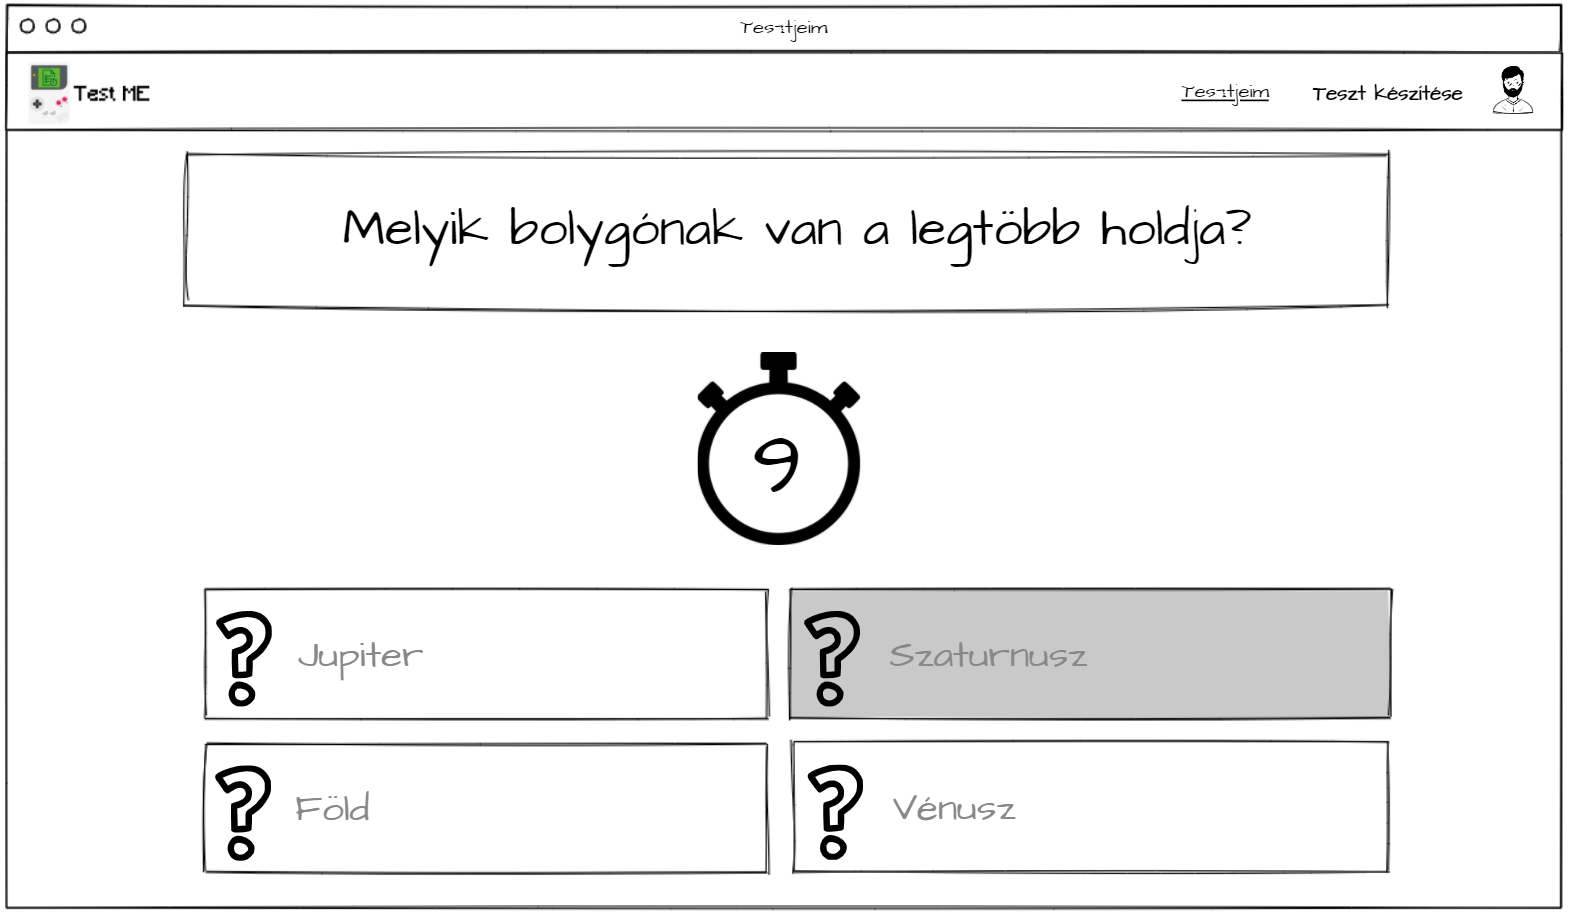
\includegraphics[width=\linewidth]{images/test1_wireframe.png}
    \caption{Feltett kérdés}
    \label{fig:test_question}
\end{figure}

Itt \ref{fig:test_question} egy kérdést látható teszt indítás után. Minden kérdésnél egy stopper órában láthatjuk hány másodpercünk van még válaszolni.

\begin{figure}[H]
    \centering
    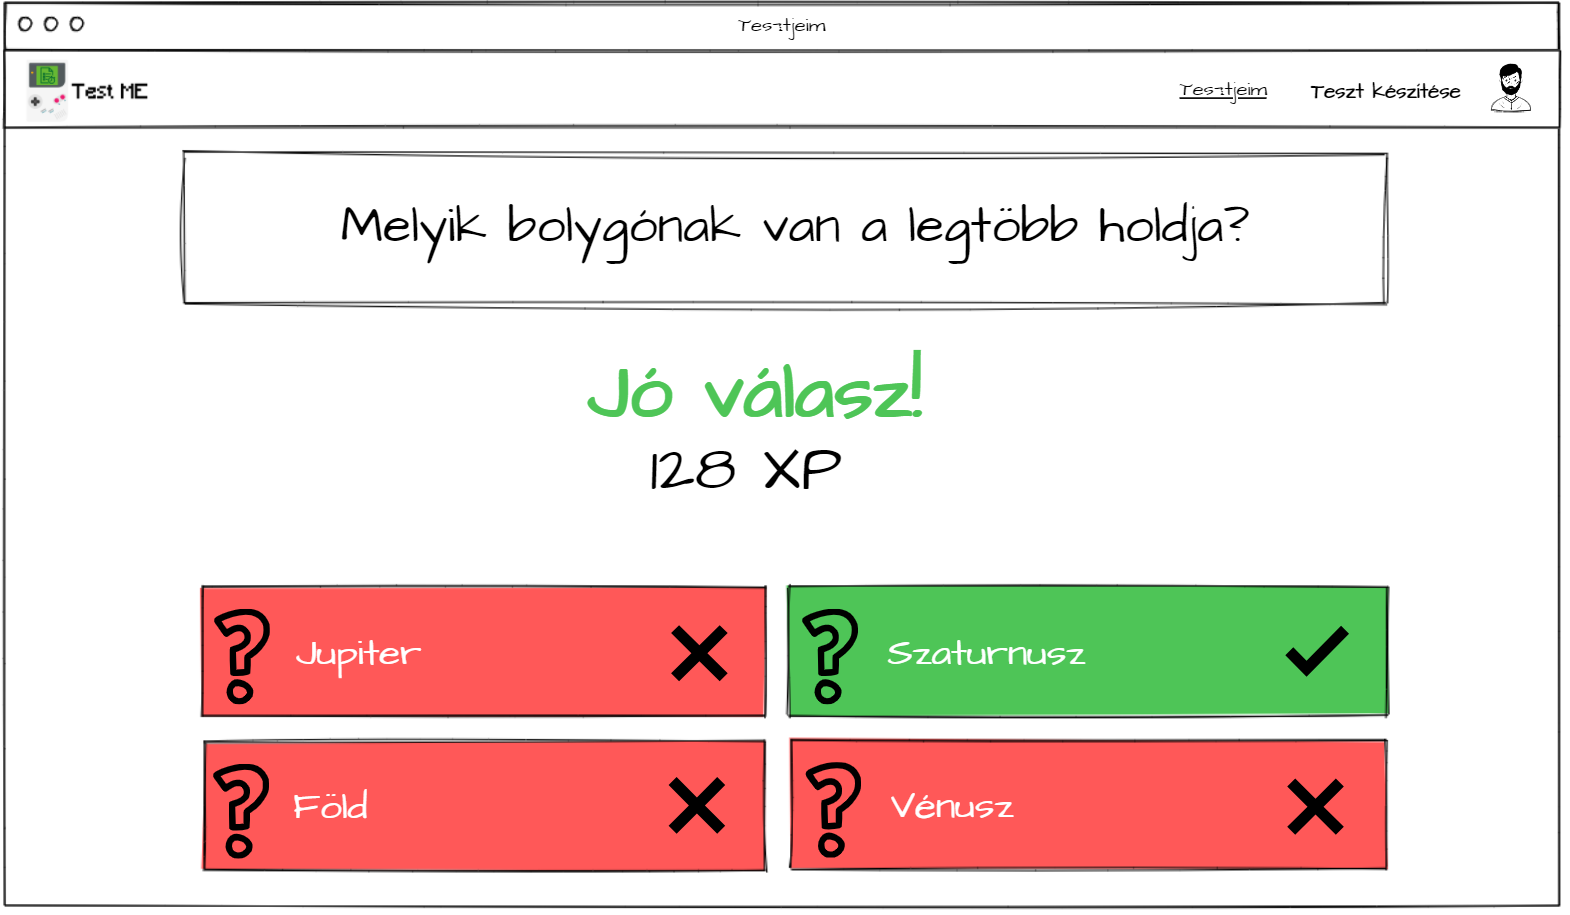
\includegraphics[width=\linewidth]{images/test2_wireframe.png}
    \caption{Válasz a kérdésre}
    \label{fig:test_answer}
\end{figure}

Válasz adás után pedig láthatjuk \ref{fig:test_answer} hogy ha válaszolunk egy kérdésre akkor melyik volt a jó és hogy válaszunk rossz vagy jó.

\begin{figure}[H]
    \centering
    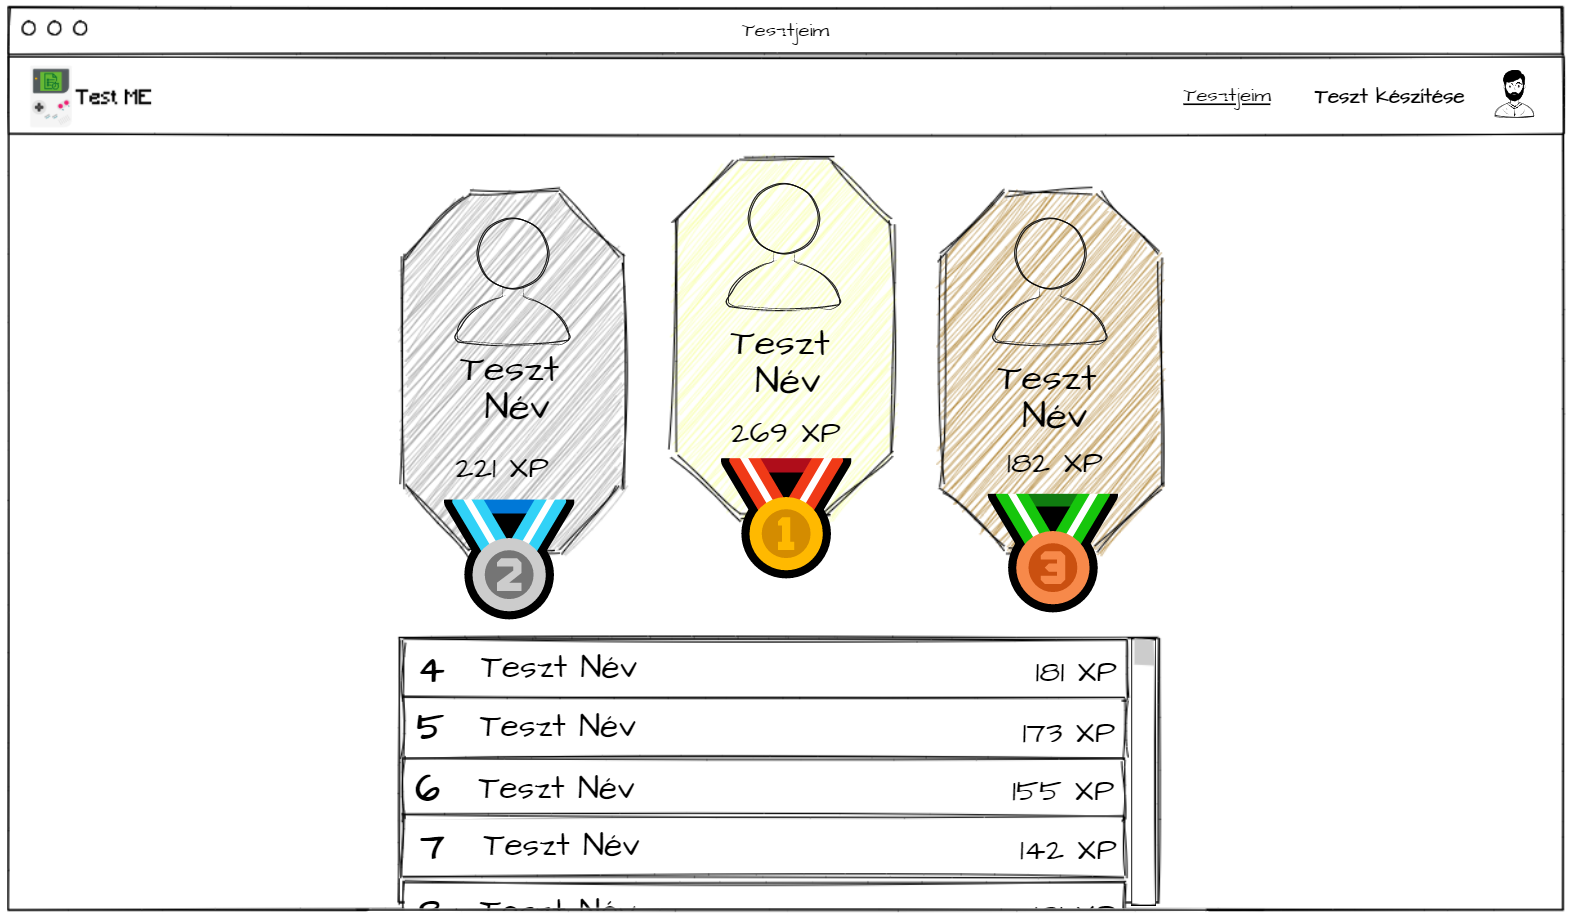
\includegraphics[width=\linewidth]{images/test3_wireframe.png}
    \caption{Teszt eredmény}
    \label{fig:test_finished}
\end{figure}

Miután válaszoltunk minden kérdésre láthatjuk mennyi pontot gyűjtöttünk és hogy kik lettek a legjobbak. \ref{fig:test_finished}


\Section{Funkciók}

\begin{itemize}
    \item {Bejelentkezés/Regisztráció}
          \begin{addmargin}[\parindent]{0pt}
              Az weboldal megnyitásakor a felhasználónak be kell jelentkeznie vagy egy helyes e-mail címmel és egy kellően biztonságos jelszóval, regisztrálni kell ha használni szeretné az oldalt.
          \end{addmargin}
    \item {Tesztkészítés}
          \begin{addmargin}[\parindent]{0pt}
              Kahoot!-hoz hasonló teszt készítési felületet szeretnék létrehozni ahol az elkészített teszteket hozzá lehet rendelni diákokhoz és ezután kitölthetik azokat.
          \end{addmargin}
    \item {Pontgyűjtés}
          \begin{addmargin}[\parindent]{0pt}
              Minden regisztrált felhasználó rendelkezik majd egy szinttel és egy bizonyos pontszámmal, amelyet a tesztek kitöltésével szerezhetnek.
          \end{addmargin}
    \item {Ranglista}
          \begin{addmargin}[\parindent]{0pt}
              Ranglista a teszt teljes kitöltését követően alakul ki a legtöbbet szerzett pontok alapján.
          \end{addmargin}
    \item {Felhasználói szerepkörök kezelése}
          \begin{addmargin}[\parindent]{0pt}
              Különböző szerepkörök lennének amik azzal bírnának hogy egy tanár jogosultságú felhasználó hozhat létre tesztet és hozzá rendelheti diákokhoz. A diák pedig csak kitölthetné azt.
          \end{addmargin}
    \item {Tesztek diákhoz rendelése}
          \begin{addmargin}[\parindent]{0pt}
              Teszt létrehozása során email cím vagy valamilyen más egyedi azonosító segítségével hozzá lehetne rendelni diákokhoz a tesztet és így értesülnének róla hogy ki kell tölteniük.
          \end{addmargin}
    \item {Összes hozzárendelt teszt megtekintése}
          \begin{addmargin}[\parindent]{0pt}
              Diákként meg lehet nézni az összes olyan tesztet amit valaki hozzá rendelt a profilhoz. És ezzel együtt a régiek eredményét is, hogy az hogy sikerült mindenkinek.
          \end{addmargin}
\end{itemize}

% TODO: Külön szakaszban érdemes lenne a szerepköröket is részletezni, az azokhoz tartozó jogosultságokat. (Lehet inkább ehhez tartozna inkább a use case diagram.)

\subsection{Szerepkörök és használati eset}

Itt látható egy kezdetleges használati eset-modell (use case diagram) ebben benne van a felhasználók információs igényeinek elemzése, funkcionális követelmények elemzése és a modell tartalmazza a rendszerrel szemben támasztott felhasználói követelményeket.
Látszik hogy kik (esetünkben tanár és diák) és mire akarják használni a rendszert.

\begin{figure}[h]
    \centering
    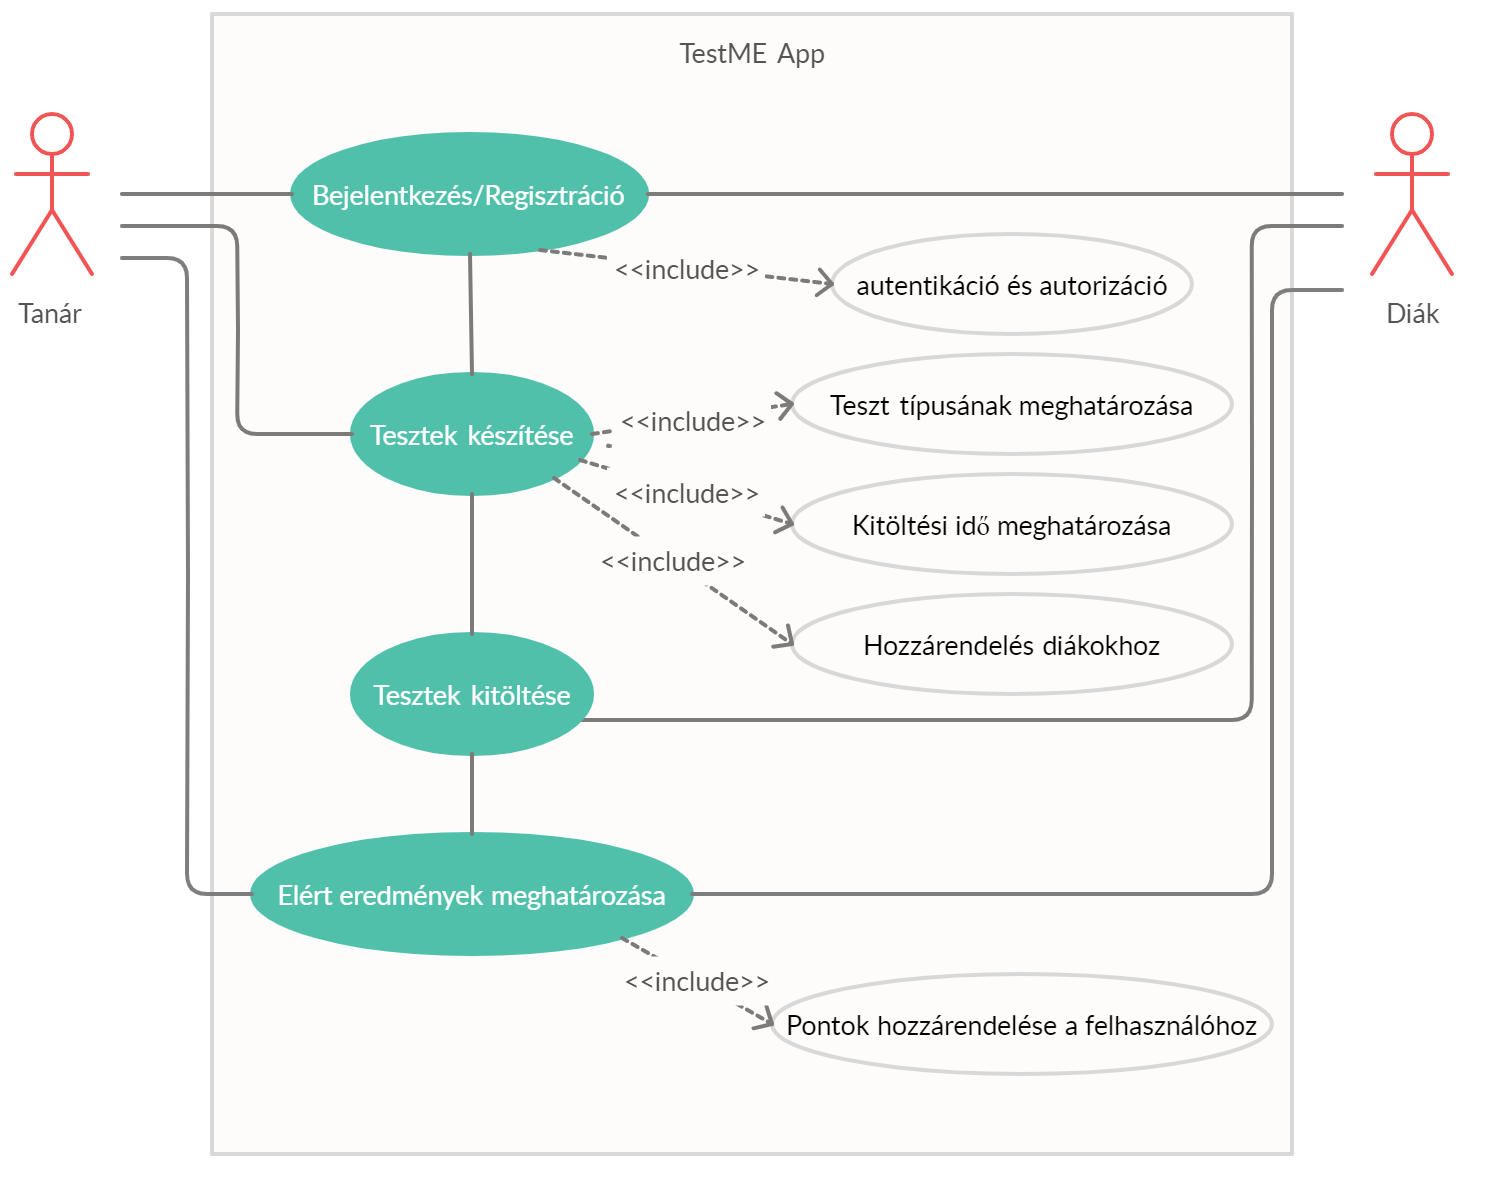
\includegraphics[width=12cm]{images/use_case.png}
    \caption{Használati eset-modell}
\end{figure}

\vspace{5mm}

Az oldalon lévő minden funkciót csak regisztráció vagy bejelentkezés után lehet használni. Ez azért fontos hiszen csak így lehet a felhasználónak tesztet küldeni és kitöltés után csak így lehet hozzáadni a profiljához a pontokat és megjeleníteni a nevét a ranglistán.

\vspace{5mm}

\noindent Regisztrálni lehet majd tanár és diákként. Ez a kettő azért van szétválasztva hogy a diákok jogosultsági körét korlátozni lehessen, például hogy egy diák ne írhasson egy tesztet és rendelje hozzá a tanárjához. Tehát ez a két funkció csak tanárok számára elérhető.

\subsubsection{Tanár szerepkör}
Egy tanár tud teszteket létrehozni és azokat hozzárendelni diákokhoz.

\subsubsection{Diák szerepkör}
Annyiban tér el a tanárétól hogy nem tud tesztet létrehozni csak a hozzárendelteket megtekinteni és kitölteni.


\Section{Adatmodell}

Az adatokat egyed-kapcsolat diagrammon ábrázoltam így a teljes kép könnyebben áttekinthető ezen rendszervázlat alapján.

\begin{figure}[H]
    \centering
    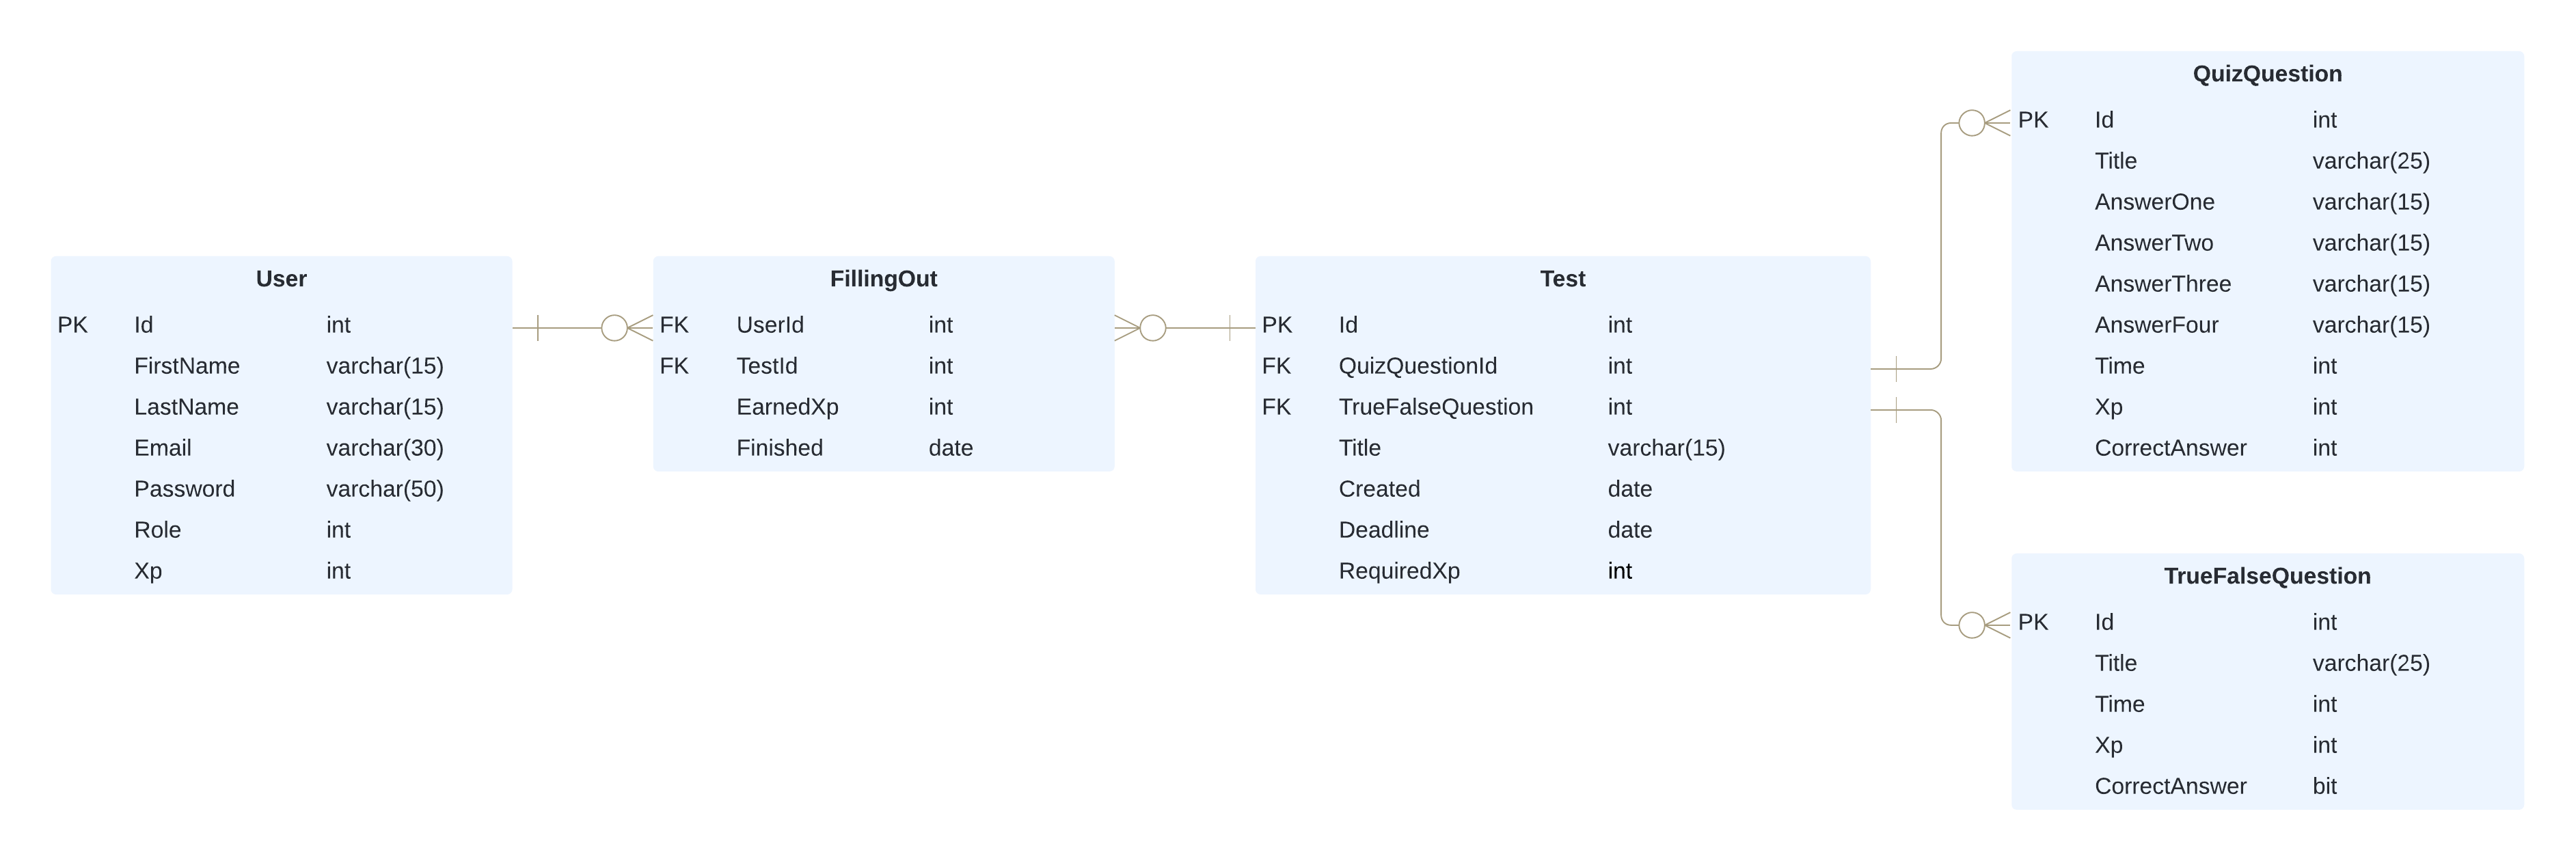
\includegraphics[width=\linewidth]{images/TestME_ER.png}
\end{figure}

A diagramm 5 táblából áll, melyek az alábbiak:
\begin{itemize}
    \item {User}
          \begin{addmargin}[\parindent]{0pt}
              Ez a tábla egy felhasználót reprezentál akinek az alap létfontosságú adatait bekérjük regisztrációkor, ilyen például a név, email cím, jelszó. Majd ezen felül még meg kell határoznia milyen szerepkörben szeretné használni az oldalt és miután töltött ki tesztet növekedni fog az xp-je mennyisége így van egy Xp adattag is.
          \end{addmargin}

    \item {Test}
          \begin{addmargin}[\parindent]{0pt}
              A Test tábla egy tanár által készített tesztet reprezentál. Egy teszten belül két típusú kérdés lehet az egyik a kvíz a másik az igaz/hamis. Ezenkívül benne van a teszt címe, hogy mikor készült és hogy mi a kitöltési határidő.
          \end{addmargin}

    \item {Question}
          \begin{addmargin}[\parindent]{0pt}
              A Question egy kérdés adatait tárolja amibe beletartozik a kérdés, a négy válasz, az idő, hogy mennyi pontot ér és hogy melyik a helyes válasz.
          \end{addmargin}

    \item {Answer}
          \begin{addmargin}[\parindent]{0pt}
              Ez a tábla egy kérdés válaszát tárolja el. Ebben a táblában benne van az előbb említett táblák azonosítója, emellett hogy mennyi pontot kapott a felhasználó a kérdésre.
          \end{addmargin}

    \item {UsersTest}
          \begin{addmargin}[\parindent]{0pt}
              Ez egy kapcsolótáblát képez a Test és a User tábla között. A kapcsolótábla azonosítója a két idegen kulcsból képzett összetett kulcs lesz. Tehát ebbe benne lesz a Test és User tábla idegen kulcsa. Erre azért van szükség hogy le tudjuk kérni hogy egy felhasználóhoz melyik tesztek tartoznak.
          \end{addmargin}

\end{itemize}

\Section{API}

Az alábbi endpointokat szeretném használni az adatok lekérésére és tárolására:
\subsection{Felhasználók}
\begin{itemize}[label={$\bullet$}, topsep=0pt, itemsep=0pt, leftmargin=15pt]
    \item[] {\url{api/users:}}
          \begin{addmargin}[\parindent]{0pt}
              Ezen az endpoint-on tudunk lekérni egy felhasználót bejelentkezéskor egy \url{GET} hívással és regisztrációkor ide tudjuk elküldeni az adatait \url{POST}-tal. Bejelentkezéskor a felhasználó email címét és jelszavát elküldve kikeressük hogy valóban létező, mentett email címet és jelszót küldött el és visszaküldjük a felhasználó adatait.

              \begin{json}
{
    "Email": "teszt@teszt.hu",
    "Password": "jelszo000"
}
              \end{json}

              Visszaküldött adatok:
              \begin{json}
{
    "id": 3,
    "roleId": 0,
    "firstName": "Makszimus",
    "lastName": "Levente",
    "email": "teszt@teszt.hu",
    "password": "jelszo000",
    "xp": 0,
    "registrationDate": "2021-01-22T00:00:00",
    "activated": false
}
            \end{json}

              Regisztrációkor pedig elküldődnek a felhasználó adatait és bejelentkezteti az oldal. Az elküldött adatok az alábbiak:

              \begin{json}
{
    "RoleId": 0,
    "FirstName": "Makszimus",
    "LastName": "Levente",
    "Email": "teszt@teszt.hu",
    "Password": "jelszo000"
}
            \end{json}

              Valamint lehet egy felhasználó adatait módosítani, \url{PUT} és törölni, \url{DELETE} hívással ugyan azon az endpointon: \url{api/users/id}.
          \end{addmargin}
\end{itemize}

\subsection{Teszt}
\begin{itemize}[label={$\bullet$}, topsep=0pt, itemsep=0pt, leftmargin=15pt]
    \item[] {\url{api/tests:}}
          \begin{addmargin}[\parindent]{0pt}
              Ha a diák ki akarja tölteni a tesztet innen tudjuk lekérni a kérdésekkel együtt. Illetve ha valaki készít egyet akkor ide küldi el az újat.
              Egy elkészített teszt így néz ki ha elküldjük \url{POST}-tal:
              \begin{json}
{
    "Title": "Mesterséges intelligencia alapok 2 teszt",
    "Created": "2021-01-12",
    "Deadline": "2021-01-22",
    "Creator": "Makszimus Levente",
    "Description": "Mesterséges intelligencia alapok második zárthelyi dolgozat",
    "Questions": [
        {
            "Problem": "Ha csinálnánk egy csoportos IQ tesztet egy tankör hallgatóival mennyi lenne az átlag?",
            "AnswerOne": "110",
            "AnswerTwo": "120",
            "AnswerThree": "130",
            "AnswerFour": "140",
            "Time": 10,
            "Xp": 5,
            "CorrectAnswer": 0
        },
        {
            "Problem": "A Turing-teszt teljesítéséért járó arany medál a díj kitűzőjét, Hugh Loebnert ábrázolja?",
            "AnswerOne": "true",
            "AnswerTwo": "false",
            "Time": 5,
            "Xp": 3,
            "CorrectAnswer": 0
        }
    ]
}
                \end{json}

              Ha pedig a felhasználó ki szeretné tölteni akkor egy \url{GET} hívással a \url{/api/tests/3} endpontra ezt kapnánk:
              \begin{json}
{
    "id": 3,
    "description": "Ez egy új teszt",
    "creator": "Makszimus Levente",
    "title": "Mesterséges intelligencia alapok első zárthelyi dolgozat",
    "created": "2021-01-12T00:00:00",
    "deadline": "2021-01-22T00:00:00",
    "questions": [
        {
            "id": 5,
            "problem": "Ha csinálnánk egy csoportos IQ tesztet egy tankör hallgatóival mennyi lenne az átlag?",
            "answerOne": "110",
            "answerTwo": "120",
            "answerThree": "130",
            "answerFour": "140",
            "time": 10,
            "xp": 5,
            "correctAnswer": 0
        },
        {
            "id": 6,
            "problem": "A Turing-teszt teljesítéséért járó arany medál a díj kitűzőjét, Hugh Loebnert ábrázolja?",
            "answerOne": "true",
            "answerTwo": "false",
            "answerThree": null,
            "answerFour": null,
            "time": 5,
            "xp": 3,
            "correctAnswer": 0
        }
    ]
}
                    \end{json}
          \end{addmargin}
\end{itemize}


\subsubsection{Válaszok}
\begin{itemize}[label={$\bullet$}, topsep=0pt, itemsep=0pt, leftmargin=15pt]
    \item[] {\url{api/tests/answers:}}
          \begin{addmargin}[\parindent]{0pt}
              Itt egy teszt kérdés válasza tárolódik amely kötődik a teszthez és magához a kérdéshez.

              \begin{json}
[
    {
        "QuestionId": 1,
        "UsersTestId": 2,
        "Time": 5,
        "userAnswer": 4
    }
]
                \end{json}
          \end{addmargin}
\end{itemize}

\subsection{Felhasználó tesztjei}
\begin{itemize}[label={$\bullet$}, topsep=0pt, itemsep=0pt, leftmargin=0pt]
    \item[] {\url{api/UsersTests:}}
          \begin{addmargin}[\parindent]{0pt}
              Ha egy diák meg akarja nézni a saját tesztjeit hogy miket kell kitöltenie és miket töltött eddig ki akkor azt innen tudjuk lekérdezni. Ezáltal kiírathatjuk őket, azokkal az információkkal hogy befejezték-e már és hogy mennyi pontot kaptak általa. A lekérés a felhasználó id-jának elküldésével történne, és ezt kell visszakapnunk:

              \begin{json}
{
    "id": 1,
    "userId": 1,
    "testId": 1,
    "test": {
        "id": 1,
        "title": "Mesterséges intelligencia alapok 2 teszt",
        "created": "2021-01-12T00:00:00",
        "deadline": "2021-01-22T00:00:00",
        "questions": [
            {
                "id": 1,0
                "title": "Ha csinálnánk egy csoportos IQ tesztet egy tankör hallgatóival mennyi lenne az átlag?",
                "answerOne": "110",
                "answerTwo": "120",
                "answerThree": "130",
                "answerFour": "140",
                "time": 10,
                "xp": 5,
                "correctAnswer": 0
            },
            {
                "id": 2,
                "title": "A Turing-teszt teljesítéséért járó arany medál a díj kitűzőjét, Hugh Loebnert ábrázolja?",
                "answerOne": "true",
                "answerTwo": "false",
                "answerThree": null,
                "answerFour": null,
                "time": 5,
                "xp": 3,
                "correctAnswer": 0
            }
        ]
    },
    "finished": "2021-01-13T00:00:00",
    "earnedXp": 6
}
                \end{json}

              Valamint amikor egy felhasználó befejezi a tesztkitöltést akkor megjelenik egy rangsor hogy ki hány pontot ért el ehhez le kell kérni az összes játékost akik kitöltötték az a tesztet. Ezt megtehetjük a \url{api/UsersTests/test/id} endpoint-on.
          \end{addmargin}
\end{itemize}

